\documentclass{article}
\usepackage[utf8]{inputenc}
\usepackage{times}
\usepackage{graphicx}
\usepackage[margin=0.75in]{geometry}
\usepackage{hyperref}
\renewcommand{\baselinestretch}{1.5}

\author{Bijan Varjavand\\ Kevin Necochea, Grace Hao}
\title{Lab 2c: Toughness, SEM, and EDS\\Group 2d}

\begin{document}

\maketitle

\clearpage

Toughness is a material property that has to do with how much impact a material can absorb before it fractures, also knows as deformation energy. It is measured in $\frac{J}{m^3}$ or $\frac{in*lbs*F}{in^3}$. Toughness is dependent on both the hardness and ductility of a material. For example, hard materials like ceramics have lower toughness than metals due to their lower ductility - they fracture without absorbing as much energy through deformation. Materials with an FCC lattice have a constant toughness throughout their stable temperature range, but BCC materials undergo a brittle-ductile transformation once a certain temperature is reached since their lattice changes to FCC.

The two materials used were 1018 as-received steel and 6061 as-received aluminum. In order to test toughness over a range of temperatures, some samples were put in a furnace while others were immersed in liquid nitrogen. Naturally, a temperature gradient was formed as we tested them since they sat at room temperature for increasing amounts of time. The samples were impacted in the Charpy test and fractured, where data was collected based on the absorbed energy. Afterwards, the fractured samples were observed on the scanning electron microscope(SEM).SEM is able to collect such high resolution images due to the low mass and short wavelength of electrons it uses. The electrons it emits pass through both collimators and stigmators to fully control their properties before scattering on the sample. An electron dispersive x-ray spectroscopy (EDS) was done afterwards to collect data on the composition of our samples. EDS works since each element has a unique atomic structure, which generates specific patterns of peaks.

The Charpy toughness tester was calibrated to 60 ft-lbs. The samples were loaded with their indent facing away from the impact site, and their temperatures were measured beforehand with a thermocouple. Out of the 10 samples tested for both steel and aluminum, data was only collected on the samples that completely or nearly fractured from the impact. Thus resulted in the data shown in tables 1 and 2. 

Three samples were chosen to image - an Aluminum sample and two steel samples(one with a brittle fracture, one with a ductile fracture). The samples were loaded together and the TA assisted my group in collecting the images. We initially observed the samples at a resolution of 500x, and after finding a suitable spot on the sample, took two images - the first at the current magnification, and the second at 2000x. This imaging protocol was followed for samples of Aluminum, steel that underwent brittle fracture, and steel that underwent ductile fracture. Scale bars were included in the images. EDS data was collected by a separate script. After the raw data was generated, thresholding and manual input of elements needed to be done. After, the software was able to generate plots showing material composition(Fig 6). The associated table 3 shows that the steel contains 1.6\%C and 97.8\%Fe, while the aluminum contains 95.5\%Al, among other elements. Any error is from thresholding.

It can be seen that, for the FCC Aluminum, the energy absorbed remained relatively constant - all values such as 6.5, 7.5, and 8.5 lie within a single power of ten across temperatures from -62C to 117C(Table 1). We know that the aluminum underwent a ductile fracture because of the SEM images that showed significant plastic deformation at the fracture surface as well as necking. Conversely, a shift can be seen in the BCC steel as it absorbs significantly more energy at higher temperatures, growing from 4 up to 28 in the -59C to 11C temperature range(Table 2). The estimated temperature range for the ductile-brittle transition temp is between -15C and -5C. This can be seen as the inflection point in our graph(Figure 1). The literature value for the transition temperature is 5C. This is acceptably close, taking into account the significant error associated with the lab.

The main source of error in this lab is from the Charpy toughness tester. This is because the indicator dial shifted during the recording of every measurement. Our group had to infer what the values were by looking closely during the impact. This error is seen especially in the aluminum plot(Figure 2) with how much the data varied when it should have been approximately constant. The SEM had very low error, only due to small vibrations during measurement.

\clearpage

Appendix:\\

\begin{table}[h]
\centering
\caption{Charpy test data for As-Received 6061 Aluminum}
\begin{tabular}{||c | c | c | c | c | c | c | c | c||}
	\hline
	\ 							& 1 & 2 & 3 & 4 & 5 & 6 & 7 & 8\\
	\hline \hline
	Temperature		& -62 & -33 & -12 & 0 & 22 & 38 & 74 & 117\\
	Energy Absorbed& 6.5 & 6.75 & 6.8 & 5 & 7.5 & 6 & 6.5 & 8.5\\
	\hline
\end{tabular}
\end{table}

\begin{table}[h]
\centering
\caption{Charpy test data for As-Received 1018 Steel}
\begin{tabular}{||c | c | c | c | c | c||}
	\hline
	\ 							& 1 & 2 & 3 & 4 & 5\\
	\hline \hline
	Temperature		& -59 & -42 & -15 & -3 & 11\\
	Energy Absorbed	& 4 & 4 & 15 & 24 & 28\\
	\hline
\end{tabular}
\end{table}

\begin{table}[h]
\centering
\caption{EDS data}
\begin{tabular}{||c | c | c | c | c | c | c||}
	\hline
	\ 				&	C	& Fe & Al & O & Mg & Si\\
	\hline \hline
	Aluminum		& 0.88 & 0 & 95.5 & 0.78 & 1.78 & 1.06\\
	Steel			& 1.64 & 97.8 & 0 & 0 & 0 & 0.59\\
	\hline
\end{tabular}
\end{table}

\begin{figure}[h]
	\centering
	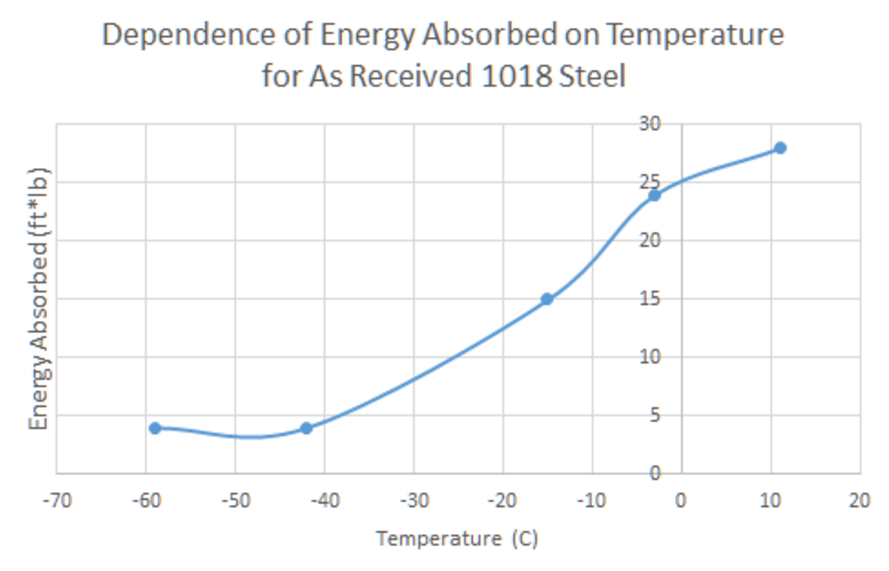
\includegraphics[scale=0.7]{2cf1.png}
	\caption{Charpy plots for Steel}
\end{figure}

\begin{figure}[h]
	\centering
	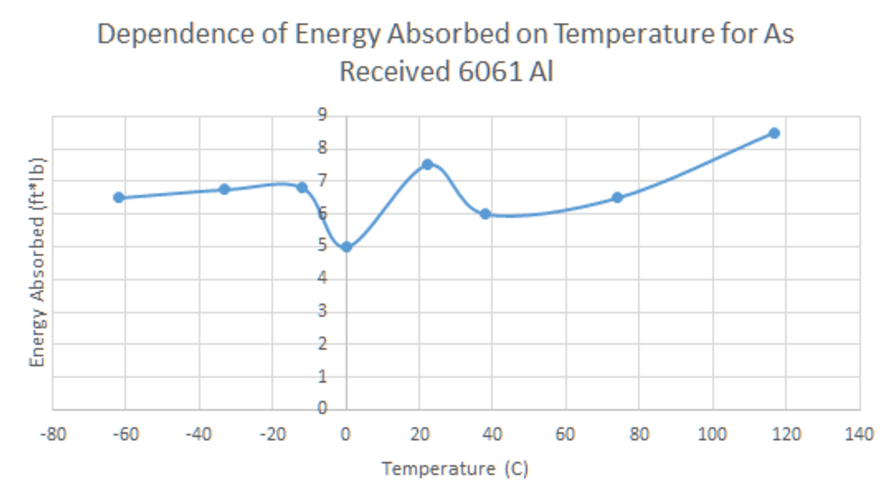
\includegraphics[scale=0.7]{2cf2.png}
	\caption{Charpy plots for Aluminum}
\end{figure}

\begin{figure}[h]
	\begin{minipage}{0.5\textwidth}
		\centering
		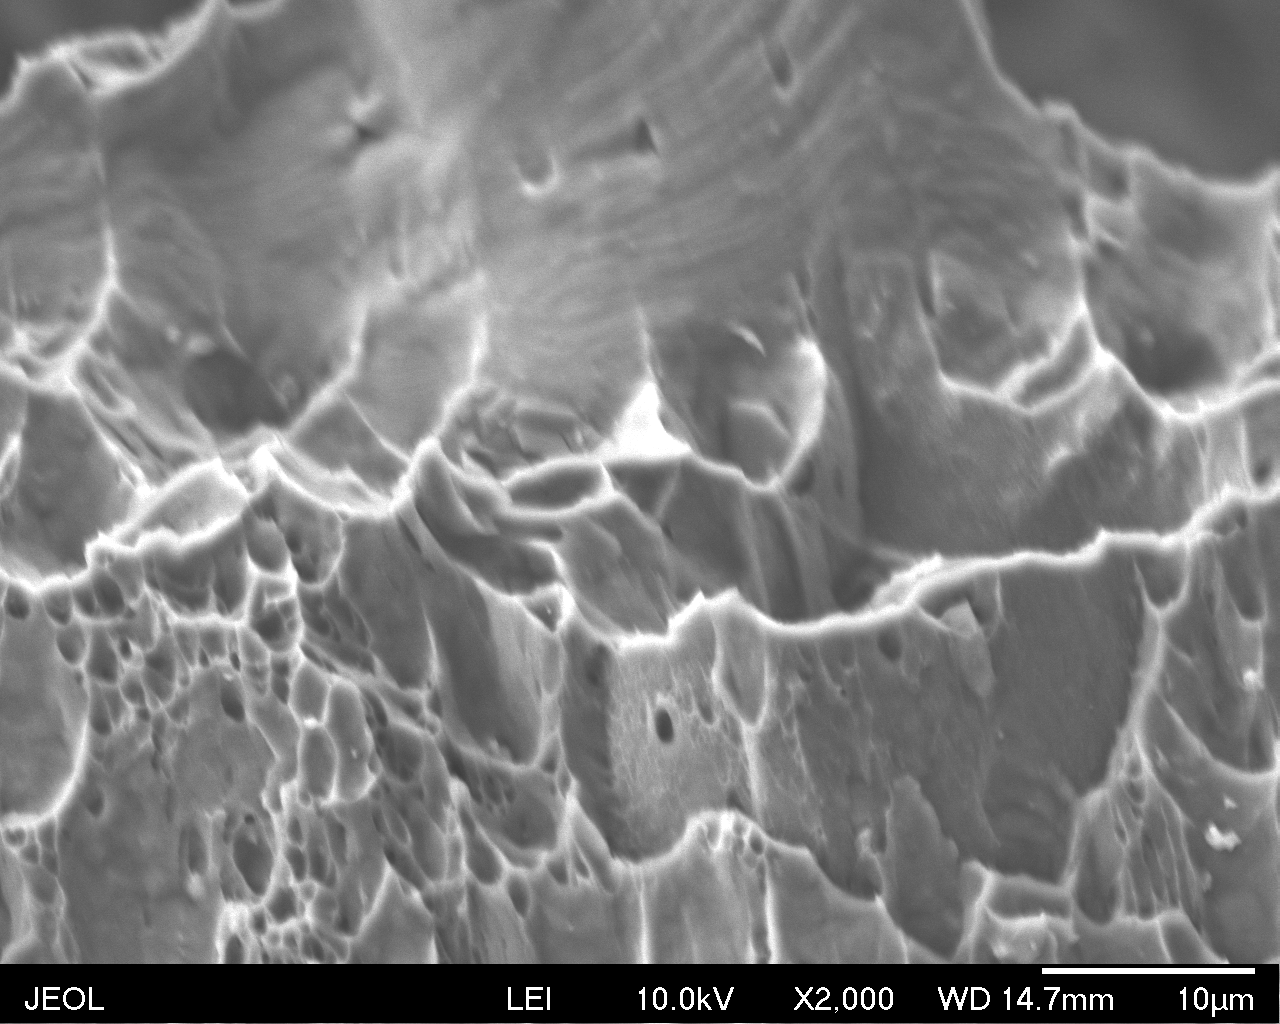
\includegraphics[scale=0.5]{Al_2kx_e.png}
	\end{minipage}
	\begin{minipage}{0.5\textwidth}
		\centering
		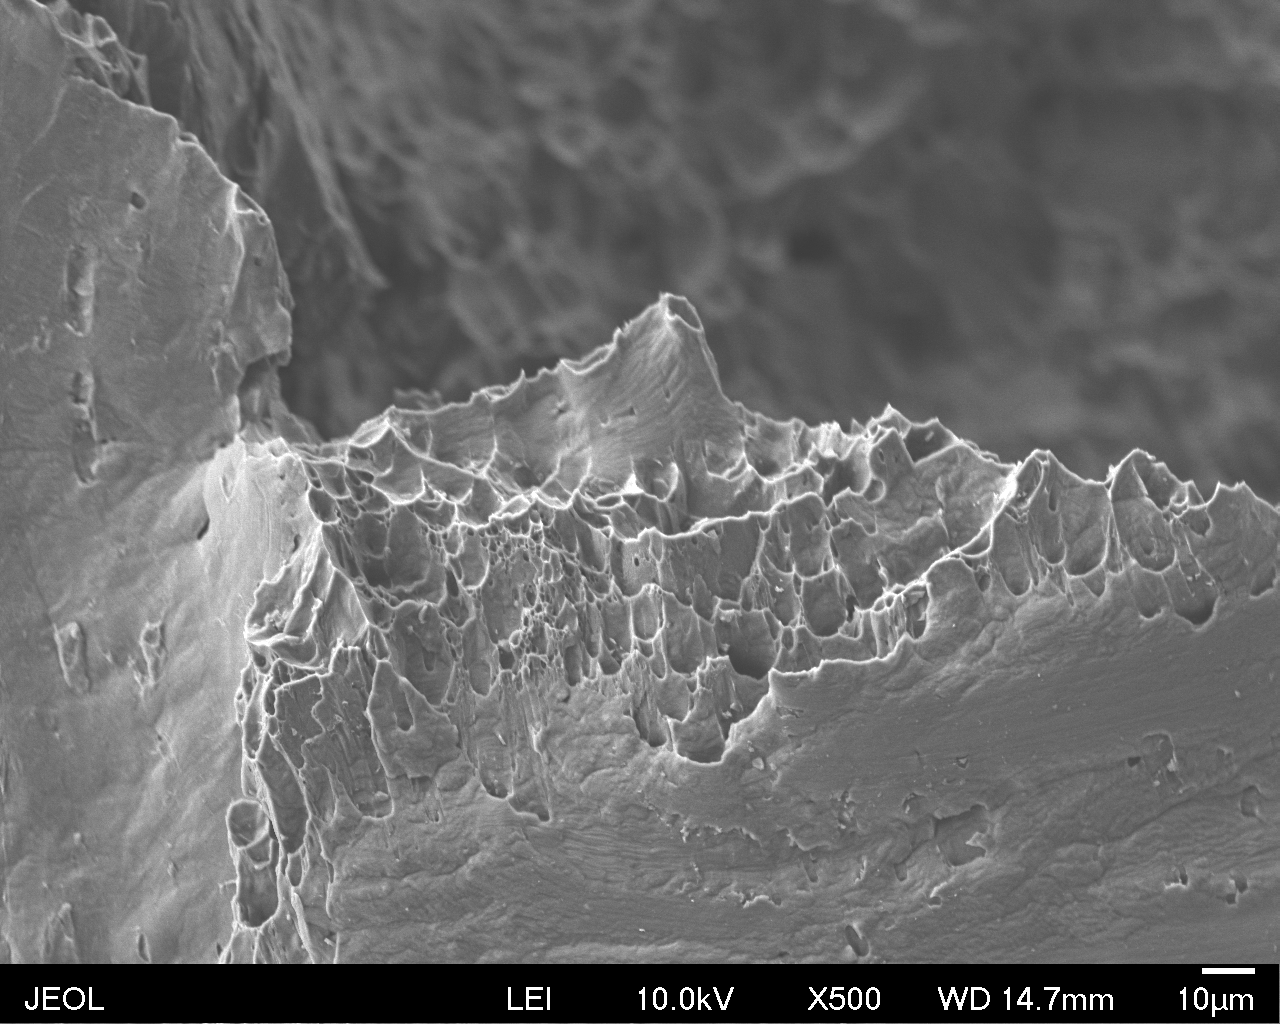
\includegraphics[scale=0.5]{Al_500x_e.png}
	\end{minipage}
	\caption{Aluminum at 2000 and 500 magnifications.}
\end{figure}

\begin{figure}[h]
	\begin{minipage}{0.5\textwidth}
		\centering
		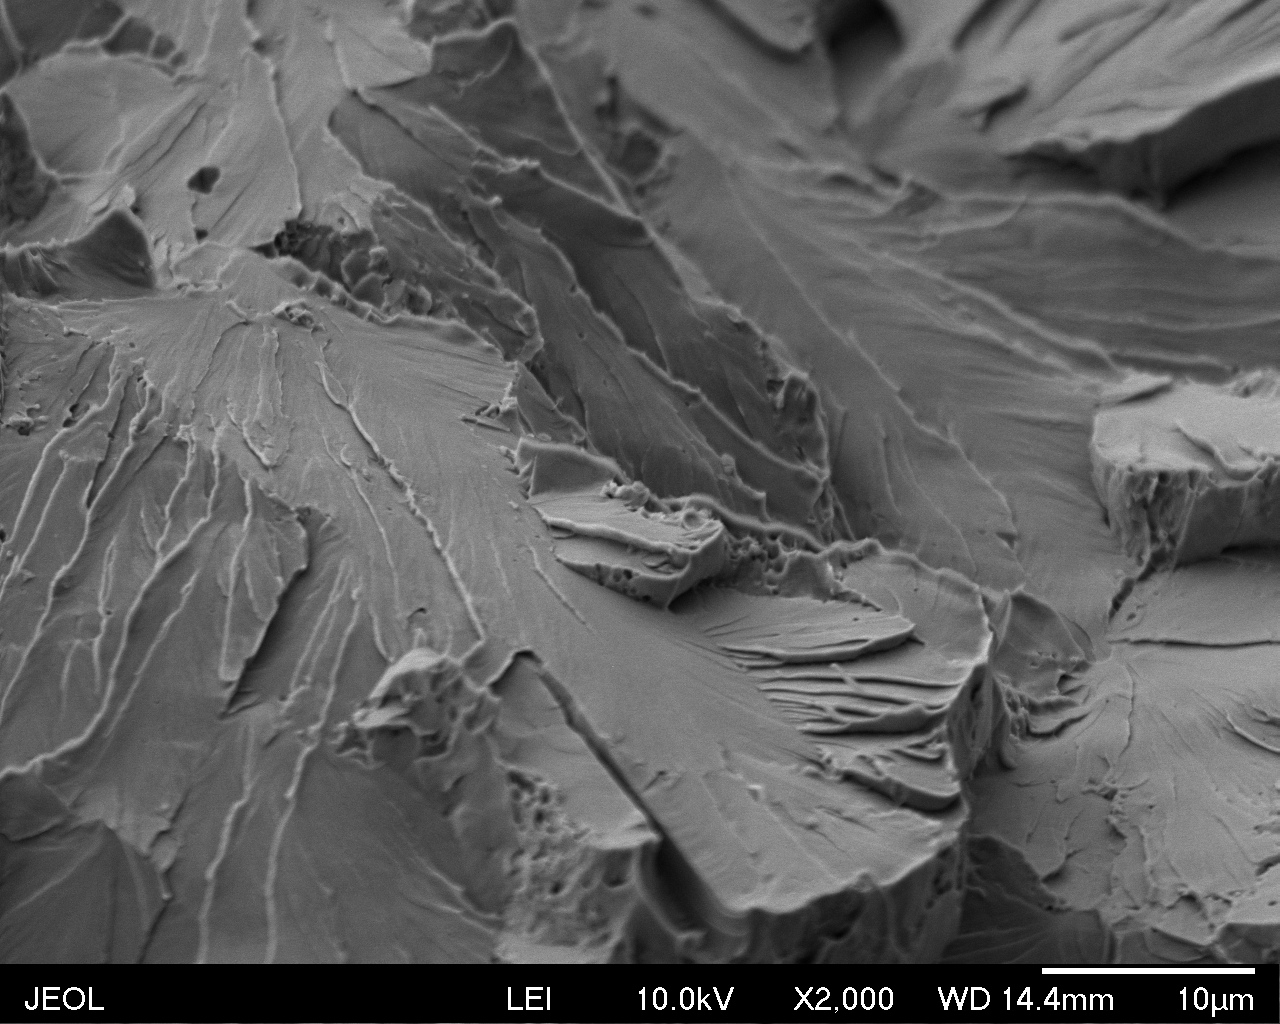
\includegraphics[scale=0.5]{steel_brittle_2kx_e.png}
	\end{minipage}
	\begin{minipage}{0.5\textwidth}
		\centering
		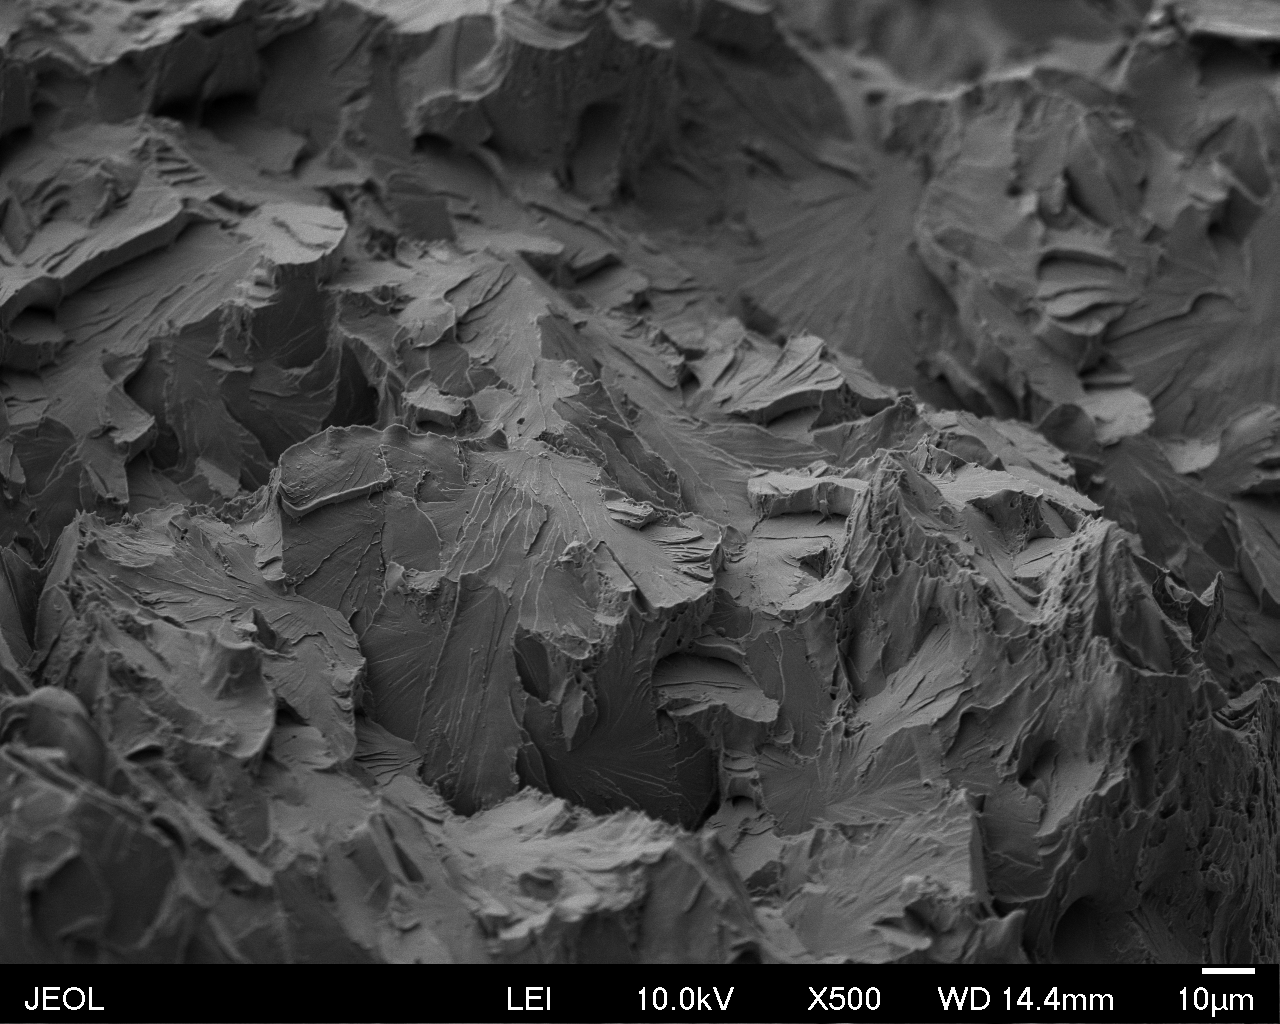
\includegraphics[scale=0.5]{steel_brittle_500x_e.png}
	\end{minipage}
	\caption{Brittle Steel at 2000 and 500 magnifications.}
\end{figure}

\begin{figure}[h]
	\begin{minipage}{0.5\textwidth}
		\centering
		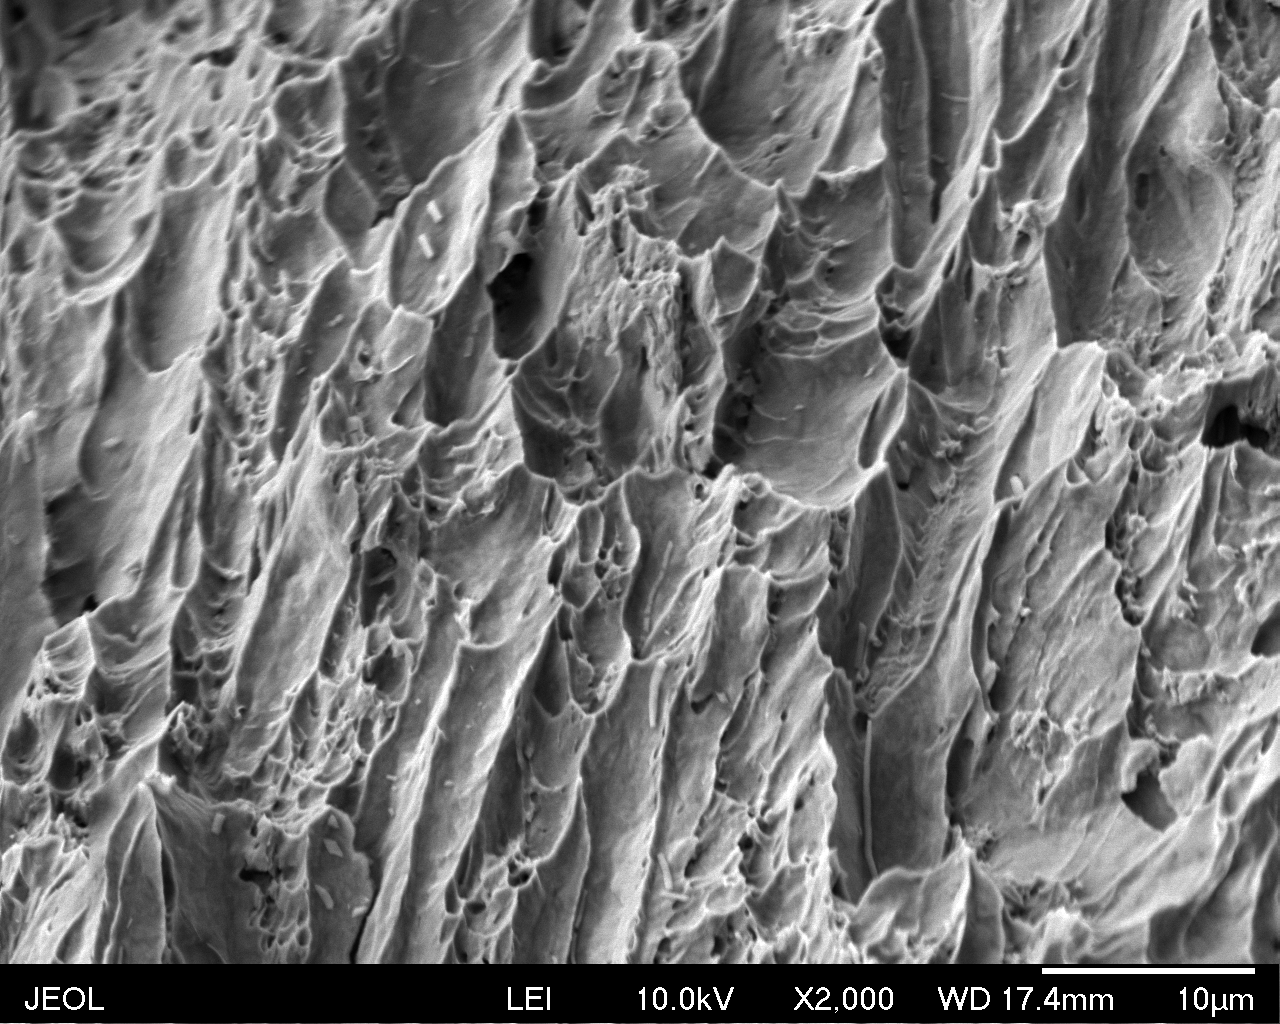
\includegraphics[scale=0.5]{steel_ductile_2kx_e.png}
	\end{minipage}
	\begin{minipage}{0.5\textwidth}
		\centering
		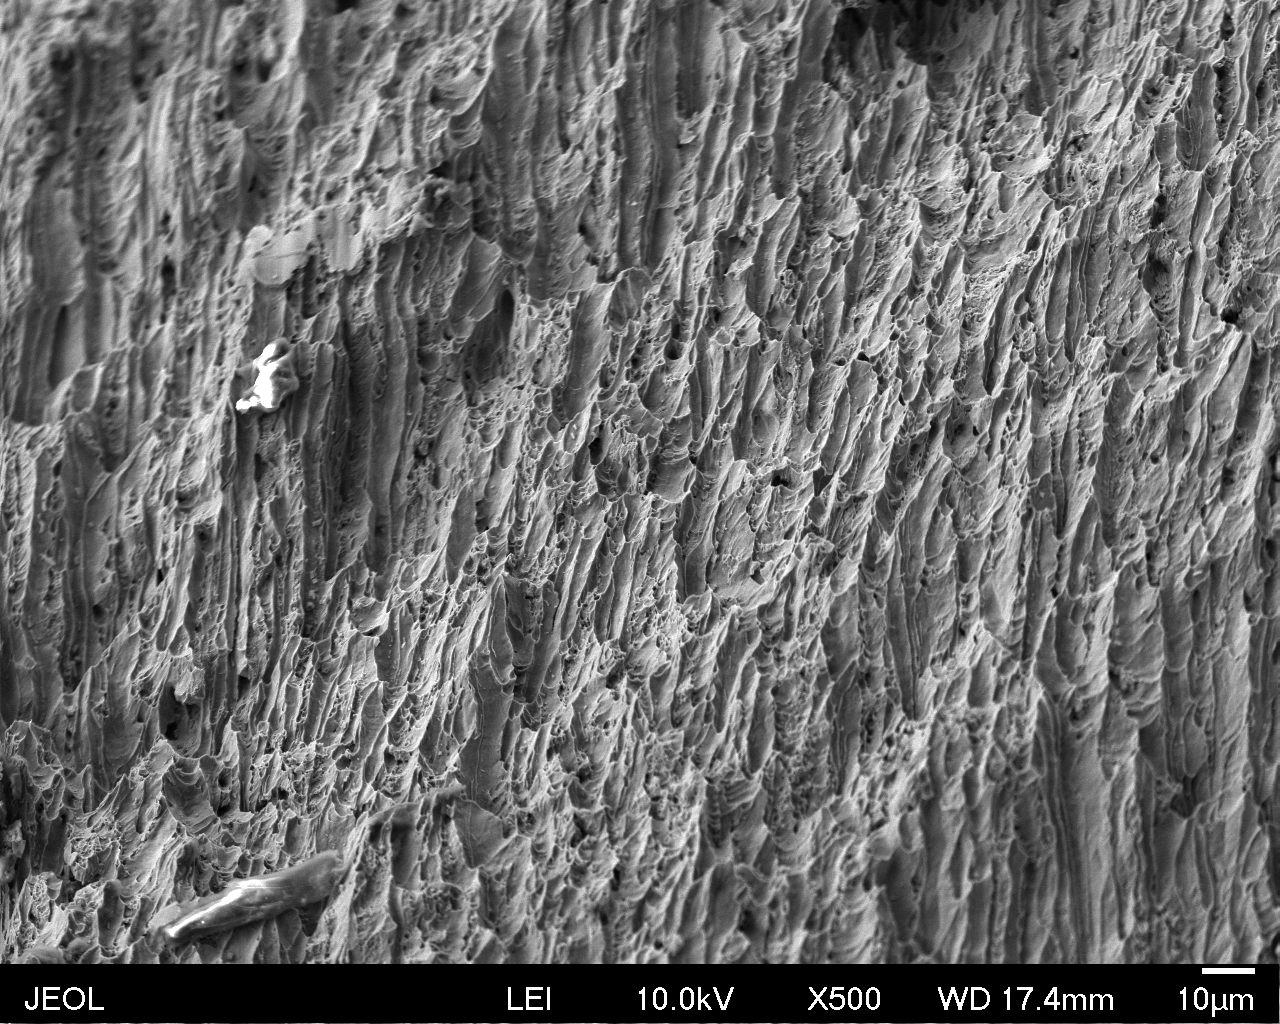
\includegraphics[scale=0.5]{steel_ductile_500x_e.png}
	\end{minipage}
	\caption{Ductile Steel at 2000 and 500 magnifications.}
\end{figure}

\begin{figure}[h]
	\centering
	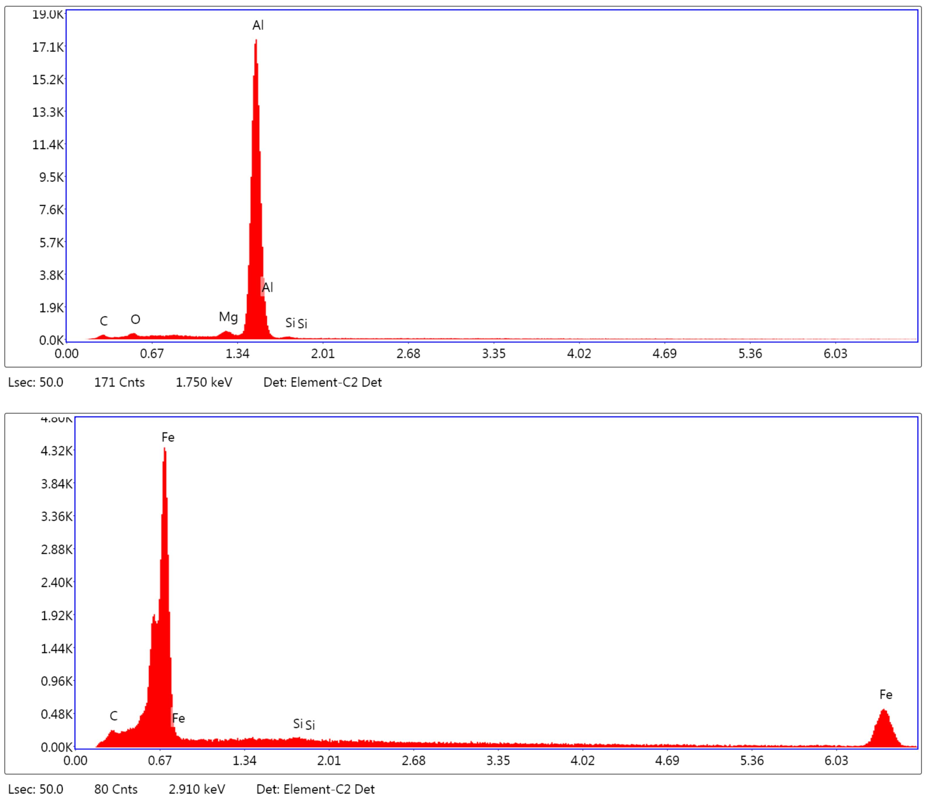
\includegraphics[scale=0.9]{2cEDS.png}
	\caption{EDS spectrum for Al and steel}
\end{figure}

\end{document}